\title{%
  An Applied Overview of Cryptography
}
\author{%
  Daniel Bosk
}
\institute[KTH/MIUN]{%
  School of Computer Science and Communication,\\
  KTH Royal Institute of Technology, Stockholm
  \and
  Department of Information and Communication Systems,\\
  Mid Sweden University, Sundsvall
}
\date{\today}

\maketitle

\mode*

\begin{abstract}
  Cryptography has a central role in security.
To fully understand how many security mechanisms can be implemented we need 
cryptography.
For this reason, we also need higher-level knowledge about what can be achieved 
with cryptography to not limit our thoughts about possible solutions.
This learning session is intended to give a high-level overview of 
cryptography: \ac{SKE}, \ac{PKE}, digital signatures, \ac{ZKP} and \ac{MPC}.
In particular, the \acp{ILO} are that you should be able to
\begin{itemize}
  \item \emph{understand} what properties can be achieved with cryptography.
  \item \emph{analyse} a situation and \emph{suggest} what cryptographic 
    properties are desirable.
\end{itemize}

We will treat
Chapter 5 in Anderson's \citetitle{Anderson2008sea}~\cite{Anderson2008sea} and
Chapter 14 in Gollmann's \citetitle{Gollmann2011cs}~\cite{Gollmann2011cs}.
To practice your understanding of these mechanisms it is recommended to do 
exercises 14.2, 14.3 and 14.7 in~\cite{Gollmann2011cs}.
We will also cover some topics from 
\citetitle{Katz-Lindell}~\cite{Katz-Lindell} and 
\citetitle{GoldreichFOC-1}~\cite{GoldreichFOC-1}.

\end{abstract}


% Since this a solution template for a generic talk, very little can
% be said about how it should be structured. However, the talk length
% of between 15min and 45min and the theme suggest that you stick to
% the following rules:  

% - Exactly two or three sections (other than the summary).
% - At *most* three subsections per section.
% - Talk about 30s to 2min per frame. So there should be between about
%   15 and 30 frames, all told.


\section{Introduction}

\subsection{History}

\begin{frame}
  \begin{itemize}
    \item The word has its origin in greek~\cite{OED2013cg}:
      \begin{description}
        \item[\ibygr{krupto's}] (\emph{kryptos}) meaning 
          hidden~\cite{OED2013c}.
        \item[\ibygr{gra'fos}] (\emph{graphos}) meaning 
          writing~\cite{OED2013g}.
      \end{description}

      \pause{}

    \item The area has been around for ages.

  \end{itemize}
\end{frame}

\begin{frame}
  \begin{itemize}
    \item Then it was an art, now it's a science.

      \pause{}

    \item People used \enquote{clever} constructions.
    \item These were thought to be secure: \enquote{How can anyone figure this 
        out?}

      \pause{}

    \item Well, it turns out that there are always a lot of people with a lot 
      of time and motivation \dots
  \end{itemize}
\end{frame}

\subsection{Kerckhoff's Principle}

\begin{frame}
  \begin{block}{A quote}
    \begin{displaycquote}[translated from French]{KerckhoffsPrinciple}\relax
      [A cryptosystem] should not require secrecy, and it should not be 
      a problem
      if it falls into the enemy hands;
    \end{displaycquote}
  \end{block}

  \pause{}

  \begin{block}{Kerckhoff's Principle}
    \begin{itemize}
      \item No security-by-obscurity
      \item The key should be the only secret
    \end{itemize}
  \end{block}
\end{frame}

\begin{frame}
  \begin{itemize}
    \item This doesn't mean we have to tell the adversary what we're using.
    \item But we shouldn't loose any security if we do.
  \end{itemize}
\end{frame}


\section{Symmetric Cryptography}

\subsection{Ciphers}

\begin{frame}
  \begin{block}{The idea}
    \begin{itemize}
      \item Alice and Bob share a (small) common secret.

        \pause{}

      \item Alice takes a message, combines it with the secret, sends it to 
        Bob.

        \pause{}

      \item If Eve captures the whatever Alice sent, she shouldn't learn 
        anything about the message.

        \pause{}

      \item Bob combines what he received with the secret and gets the message.
    \end{itemize}
  \end{block}
\end{frame}

\begin{frame}
  \begin{block}{Block-cipher encryption}
    \begin{description}
      \item[Input] A fixed-sized \emph{key} \(\Key{}\), a fixed-sized block of 
        \emph{plaintext} \(p\).
      \item[Output] A fixed-sized block of \emph{ciphertext} \(c\).
      \item[Notation] \(\Enc[\Key{}]{p} = c\)
    \end{description}
  \end{block}

  \pause{}

  \begin{block}{Block-cipher decryption}
    \begin{description}
      \item[Input] A fixed-sized \emph{key} \(\Key{}\), a fixed-sized block of 
        \emph{ciphertext} \(c\).
      \item[Output] A fixed-sized block of \emph{plaintext} \(p\).
      \item[Notation] \(\Dec[\Key{}]{c} = p\)
    \end{description}
  \end{block}
\end{frame}

\begin{frame}
  \begin{definition}\label{CryptoSystem}
    \begin{itemize}
        \item A \emph{crypto system} is a tuple \((\M, \C, \K, \E, \D)\), 
          where:
          \begin{itemize}
            \item \(\M\) is a finite set of \emph{plaintexts} or messages,
            \item \(\C\) is a finite set of \emph{ciphertexts},
            \item \(\K\) is the \emph{keyspace}, a finite set of keys.
            \item \(\E\) and \(\D\) are the sets of encryption and decryption
              rules, respectively.
          \end{itemize}

          \pause{}

        \item For every \(k\in \K\) there is a \(\Enc[k]{}\in \E\) and 
          \(\Dec[k]{}\in \D\) such that
          \begin{itemize}
            \item \(\Enc[k]{}\colon \M\to \C\) and \(\Dec[k]{}\colon \C\to 
                \M\) are functions and
            \item \(\Dec[k]{\Enc[k]{m}} = m\) for all plaintexts \(m\in 
                \M\).
          \end{itemize}
      \end{itemize}
  \end{definition}
\end{frame}

\begin{frame}
  \begin{definition}[Shift Cipher]\label{ShiftCipher}
    \begin{itemize}
      \item Let \(\M = \C = \K = \Z_{29}\)
      \item For each \(k\in \K\) we define
        \begin{align}
          \nonumber
          \Enc[k]{m} &= (m + k) \bmod 29, m\in \M, \text{\ och } \\
          \nonumber
          \Dec[k]{c} &= (c - k) \bmod 29, c\in \C.
        \end{align}
    \end{itemize}
  \end{definition}

  \pause{}

  \begin{example}
    \begin{itemize}
      \item \(\Enc[3]{7} = 7+3 \bmod 29 = 10\)\hfill h\(\to\)J
      \item \(\Enc[3]{4} = 4+3 \bmod 29 = 7\)\hfill e\(\to\)G
      \item \(\Enc[3]{9} = 9+3 \bmod 29 = 12\)\hfill j\(\to\)L
    \end{itemize}
  \end{example}
\end{frame}

\begin{frame}
  \begin{exercise}
    \begin{itemize}
      \item What do we have to do to set this up between two parties, say Alice 
        and Bob?
      \item What problems do we have to solve?
    \end{itemize}
  \end{exercise}
\end{frame}

\begin{frame}
  \begin{definition}[\Acl{PRP}, \acs{PRP}]
    \begin{itemize}
      \item Let \(F\colon \{0,1\}^s\times \{0, 1\}^n\to \{0,1\}^n\).
      \item \(F\) is \iac{PRP} if
        \begin{enumerate}
          \item for any \(k\in \{0, 1\}^s\), \(F\) is a bijection;
          \item for any \(k\in \{0, 1\}^s\), we can \enquote{efficiently} 
            evaluate \(F_k(x)\);
          \item for all \enquote{efficient} distinguishers \(D\),
            \[\left|\Pr[D^{F_k}(1^n) = 1] - \Pr[D^{f_n}(1^n) = 1]\right| 
              < \epsilon(s)\] if we choose \(k\in \{0,1\}^s\) and the random 
            permutation \(f_n\) uniformly at random.
        \end{enumerate}
    \end{itemize}
  \end{definition}
\end{frame}

\subsection{Hash Functions}

\begin{frame}
  \begin{block}{The idea}
    \begin{itemize}
      \item We want a function which we can efficiently compute.

        \pause{}

      \item However, it shouldn't be possible to find its inverse.
    \end{itemize}
  \end{block}

  \pause{}

  \begin{example}
    \begin{description}
      \item[Easy] \(f(x) = y\)
      \item[Hard] \(f^{-1}(y) = x\)
    \end{description}
  \end{example}
\end{frame}

\begin{frame}
  \begin{figure}
    \subfloat[\(h\colon X\to Y\)]{%
      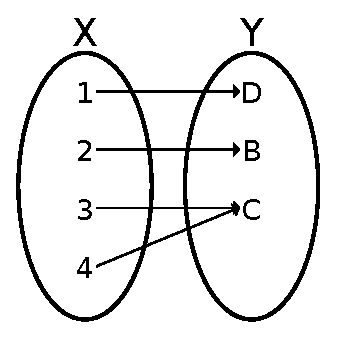
\includegraphics[height=2cm]{surjection.eps}%
    }
    \hspace{0.1\textwidth}
    \subfloat[\(h^\prime\colon X\to Y\)]{%
      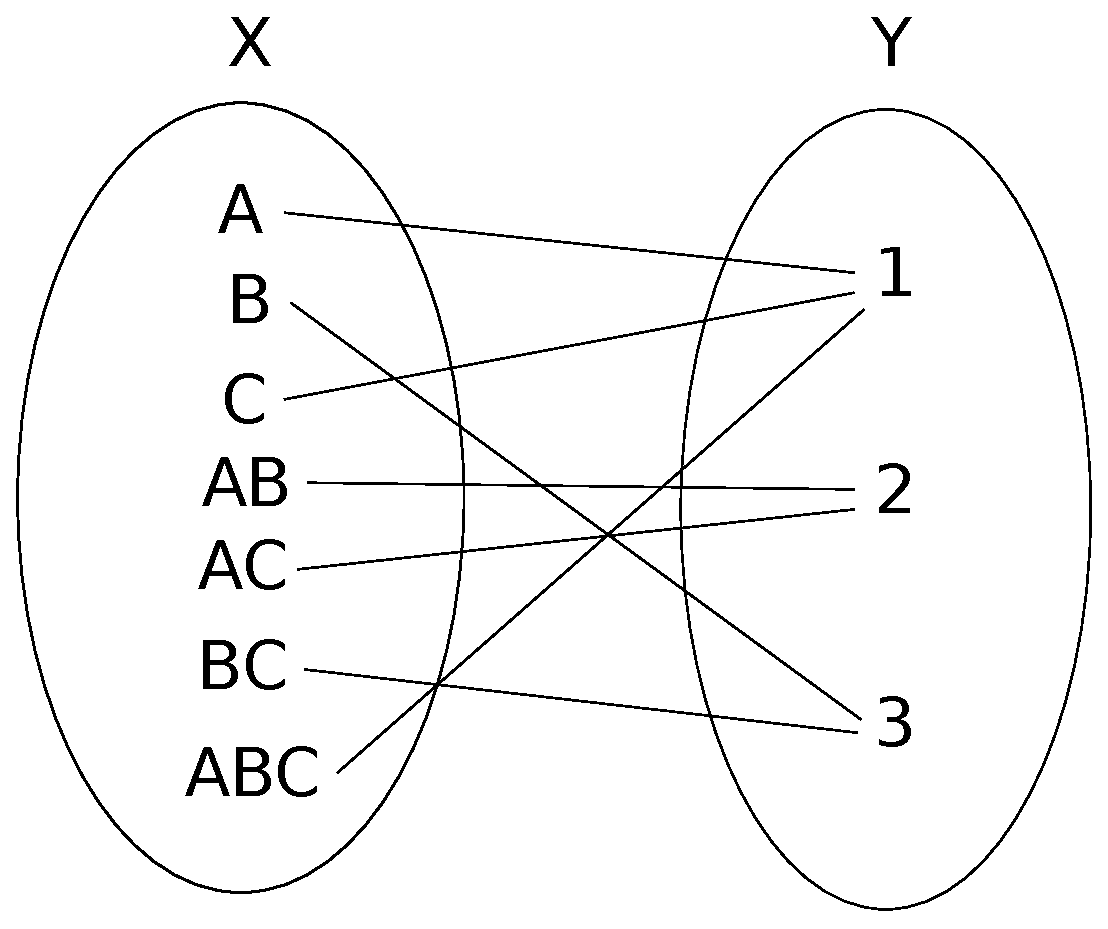
\includegraphics[height=2cm]{hashfunc.eps}%
    }
    \caption{%
      Two non-injective, surjective functions \(h\) and \(h^\prime\).
    }
  \end{figure}

  \begin{exercise}
    Could either of these two functions be one-way functions?
  \end{exercise}
\end{frame}

\begin{frame}
  \begin{definition}[One-way function]
    \begin{itemize}
      \item Let \(h\colon \{0,1\}^*\to \{0,1\}^*\).
      \item \(h\) is \emph{one-way} if
        \begin{enumerate}
          \item there exists an efficient algorithm \(A\) such that \(A(x) 
              = h(x)\);
          \item for every efficient algorithm \(A^\prime\), every positive 
            polynomial \(p(\cdot)\) and all sufficiently large \(n\)'s
            \[\Prob{A^\prime(h(x), 1^n) \in h^{-1}(h(x))} < \frac{1}{p(n)}\]
        \end{enumerate}
    \end{itemize}
  \end{definition}
\end{frame}

\begin{frame}
  \begin{example}[Implementations you might've heard of]
    \begin{itemize}
      \item MD5
      \item SHA1
      \item SHA256 (SHA-2)
      \item SHA-3
    \end{itemize}
  \end{example}
  \begin{example}[Applications]
    \begin{itemize}
      \item Verifying file content integrity
      \item Digital signatures
      \item Protect passwords
    \end{itemize}
  \end{example}
\end{frame}

\subsection{\Aclp{MAC}}

\begin{frame}
  \begin{example}
    \begin{itemize}
      \item Let \(\Enc[k]{\cdot} = \Dec[k]{\cdot} = \cdot\oplus k\bmod 2\).
        
        \pause{}

      \item Alice and Bob share \(k\).
      \item Alice sends \(\Enc[k]{m} = c\) to Bob.

        \pause{}

      \item Eve intercepts \(c\), she cannot get to \(m\).

        \pause{}

      \item Eve computes \(c^\prime = c\oplus m_E\) and passes \(c^\prime\) to 
        Bob.

        \pause{}

      \item Bob computes \(\Dec[k]{c^\prime} = \Dec[k]{c\oplus m_E} = m\oplus 
          k\oplus m_E\oplus k = m\oplus m_E\).
    \end{itemize}
  \end{example}

  \pause{}
  
  \begin{exercise}
    How can we solve this?
    Bob needs to know that Eve modified the message!
  \end{exercise}
\end{frame}

\begin{frame}
  \begin{block}{The idea: \acp{MAC}}
    \acuse{MA}
    \begin{itemize}
      \item Alice and Bob need something that Eve doesn't know how to modify.

        \pause{}

      \item If that something is tied to the message, then a modified message 
        would be detectable.
    \end{itemize}
  \end{block}

  \pause{}

  \begin{exercise}
    Any ideas on how we can construct such a thing?
  \end{exercise}
\end{frame}

\begin{frame}
  \begin{example}
    \begin{itemize}
      \item Let \(h\) be a one-way function.
        
        \pause{}
        
      \item \(h(c) = t\), Eve can also compute the hash function: \(h(c^\prime) 
          = t^\prime\).

        \pause{}

      \item A secret hash function would violate Kerckhoff's principle.

        \pause{}

      \item \(h(m) = t\), then
        \begin{itemize}
          \item \(\Dec[k]{c^\prime} = m^\prime = m\oplus m_E, h(m^\prime)\neq 
              t\).
          \item \(\Dec[k]{c} = m, h(m) = t\).
        \end{itemize}

        \pause{}
        
      \item Eve cannot compute the hash function, she doesn't have \(m\)!
        \pause{}
        \begin{itemize}
          \item Bob: But neither do I\@!
        \end{itemize}
    \end{itemize}
  \end{example}

  \pause{}

  \begin{exercise}
    Any better ideas?
  \end{exercise}
\end{frame}

\begin{frame}
  \begin{solution}
    \begin{itemize}
      \item Let \(s\) be a secret shared between Alice and Bob.

        \pause{}

      \item \(h(c\concat s) = t\), Eve doesn't know \(s\).
      \item Bob can immediately check \(h(c^\prime\concat s)\neq t\).
    \end{itemize}
  \end{solution}

  \pause{}

  \begin{alertblock}{Note}
    \begin{itemize}
      \item It requires even a bit more than this!
      \item But the idea is correct.
    \end{itemize}
  \end{alertblock}
\end{frame}

\begin{frame}
  \begin{solution}[\Acl{HMAC}, \acs{HMAC}]
    \begin{itemize}
      \item Let \(h\) be a one-way function.
      \item Let \(c\) be the ciphertext, \(s\) our \ac{MA} secret.

        \pause{}

      \item Then tag \(t = \HMAC[s]{c}\), where \[
          \HMAC[s]{c} = h\left[
            (s\oplus p_o)\concat h\left[ (s\oplus p_i)\concat c \right]
          \right],
        \] and \(p_i, p_o\) are inner and outer pads, respectively.
    \end{itemize}
  \end{solution}

  \pause{}

  \begin{alertblock}{Note}
    This is proven secure!
  \end{alertblock}
\end{frame}


\section{Public-Key Cryptography}

\begin{frame}
  \begin{itemize}
    \item Encryption and decryption
    \item Digital signatures
    \item Homomorphic properties
  \end{itemize}
\end{frame}

\subsection{Encryption and Decryption}

\begin{frame}
\end{frame}

\subsection{Digital Signatures}

\begin{frame}
\end{frame}

\subsection{Homomorphic Properties}

\begin{frame}
\end{frame}


\section{More Counter-Intuitive Things}

\subsection{Zero-Knowledge Proofs}

\begin{frame}
\end{frame}


\subsection{(Secure) Multi-Party Computation}

\begin{frame}
\end{frame}


%%%%%%%%%%%%%%%%%%%%%%

\begin{frame}[allowframebreaks]
  \printbibliography{}
\end{frame}

